\documentclass[mathserif]{beamer}
\usepackage[nofirafonts]{beamerthemefocus}
\usepackage{amsmath}


\newcommand{\refeq}[1]{Eq.~\ref{#1}}
\newcommand{\Lambdatt}[2]{\Lambda_{t+ #1, t+ #2}}
\newcommand{\Lambdat}[1]{\Lambda_{t, t+#1}}
\setbeamertemplate{caption}[numbered]

\title{Banking, Liquidity and Bank Runs in an Infinite Horizon Economy}
\author{Mark Gertler and Nobuhiro Kiyotaki \\ 
\small Presentor ~:~ Chia-Wei, Chen}

\begin{document}
    \begin{frame}
        
        \maketitle
    \end{frame}

    \section{Introduction}
    \begin{frame}
    \frametitle{Bank Run in CBDC}

    Many have discussed about the possibility of run if CBDC is issues in a closed economy.
    \begin{enumerate}[<+->]
        \item Direct deposit in central bank that is fully insured
        \item Can be interest bearing as a monetary policy
        \item Competition with commercial banks, causing disintermediation by crowding out deposits \footnote{See Fernandez-Villaverde, J., D. Sanches, L. Schilling, and H. Uhlig (2021) for a model}
        \item Financial instability (Gertler and Kiyotaki, 2015)
    \end{enumerate}
    \pause
    \vfill 
    The impact could be mitigated by proper regulations and limits on the design of CBDC.

\end{frame}

\begin{frame}
    \frametitle{Bank Run Under Foreign CBDC}

    However, if CBDC is cross-border, domestic country might be out of means.

    \begin{enumerate}[<+->]
        \item Currency substitution in high-inflation country (Calvo, 1992)
        \item CBDC is digital, easy to access using mobile devices, causing faster substitution rate 
        \item Commercial banks and domestic central bank both losses deposits, causing even more severe run and financial instability.
        \item Currency substitution could ultimately impair monetary policy (Ferrari et al. 2022)
    \end{enumerate}

\end{frame}


\begin{frame}
    \frametitle{This Paper}

    Extends DD to cross-border CBDC.

    Chooses the following foreign CBDC design
    \begin{itemize}
        \item Account-base \emph{v.s. token}
        \item Retail \emph{v.s. Wholesale}
        \item Cross border
        \item Interest-bearing
    \end{itemize}
    \pause
    The domestic country has no CBDC technology, while foreign country issues cross-border CBDC that could cause capital outflows. 

\end{frame}



    \section{Model---Main Structure}
    \begin{frame}
    \frametitle{Resource}

    \begin{itemize}
        \item Fixed capital, allocated to bank and household
        \begin{equation}
            K^b_t + K^h_t = 1
        \end{equation}
        \item Payoff for banker 
        \begin{equation}
            \begin{array}{ccc}
                \text{date}~t & & \text{date}~ t+1 \\
                K^b_t & \rightarrow & \begin{cases}
                    Z_{t+1}K^b_t \\
                    K^b_t
                \end{cases}        
            \end{array}
        \end{equation}
    \item Payoff for HH
        \begin{equation}
            \begin{array}{ccc}
                \text{date}~t & & \text{date}~ t+1 \\
                \begin{cases}
                    K^h_t \\
                    f(K^h_t)
                \end{cases} 
                & \rightarrow & \begin{cases}
                    Z_{t+1}K^h_t \\
                    K^h_t
                \end{cases}        
            \end{array}
        \end{equation} 
    \item HH needs management cost 
    \begin{equation}
        f(K^h_t) = \frac{\alpha}{2} (K^h_t)^2
    \end{equation}
    \end{itemize}
\end{frame}

    \section{Household}
    \begin{frame}
    \frametitle{Household Saving}

    \begin{itemize}
        \item HH holds nondurable goods $Z_t W^h$ each period.
        \item HH deposits their funds to (shadow) banks 
        \begin{equation}
            R_{t+1} = \begin{cases}
                \bar{R}_{t+1} & \text{if no bank run} \\
                x_{t+1}\bar{R}_{t+1} & \text{if bank run}
            \end{cases}
        \end{equation}
        all HH is distributed equal amount, unlike DD.
    \end{itemize}
\end{frame}

\begin{frame}[allowframebreaks]
    \frametitle{Household decision}
    \begin{itemize}
        \item HH maximizes lifetime utility 
        \begin{equation*}
            U_t = E_t \left(\sum_{i=0}^\infty \beta^{i} \ln{C^h_{t+i}}\right)
        \end{equation*}
        \item s.t 
        \begin{equation}
            C^h_t + D_t + Q_t K^h_t + f(K^h_t) = Z_t W^h +  R_t D_{t-1} + (Z_t + Q_t)K^h_{t-1}
        \end{equation}
        \framebreak
        \item (Assuming 0 prob of bank run) F.O.C for deposit
        \begin{equation}
            \label{eq:FOC-deposit}
            E_t \Lambda_{t, t+1}R_{t+1} = 1
        \end{equation}
        \item $\Lambda_{t, t+i}$ is defined by 
        \begin{equation}
            \label{eq:lambda}
            \Lambda_{t, t+i} = \beta^i \frac{C^h_t}{C^h_{t+i}}
        \end{equation}
        \item F.O.C for holding capital 
        \begin{equation}
            \label{eq:FOC-capital}
            E_t \Lambda_{t, t+1}R^h_{t+1} = 1
        \end{equation}
        with 
        \begin{equation}
            \label{eq:Rh}
            R^h_{t+1} = \frac{Z_{t+1} + Q_{t+1}}{Q_t + f'(K^h_t)}
        \end{equation}
    \end{itemize}
\end{frame}

\begin{frame}
    
    Remark
    \begin{itemize}
        \item If HH hold capital, \refeq{eq:FOC-capital} help determine market price. 
        \item i.e.,  Liquidation price during run. 
        \item $Q_t = E_t \Lambda_{t, t+1}(Z_{t+1} + Q_{t+1}) - f'(K^h_t)$. Market price {\bf tends to} be decreasing as $K^h_t$ increase.
        \item During bank run, HH absorbs all capital from bank, asset prices drop sharply. 
    \end{itemize}
\end{frame}

    \section{Bank}
    \begin{frame}
    \frametitle{Finite expected lifetime}
    \begin{exampleblock}{100 percent equity financing}
        To the extent bankers may face financial market frictions, 
        they will attempt to save their way out of the financing constraint by
        accumulating retained earnings in order to move toward 100 percent equity financing.  
    \end{exampleblock}

    To limit this possibility --- probability $\sigma$ of surviving, 
    hence expected lifetime $\frac{1}{1-\sigma}$ 
    \begin{enumerate}
        \item Meaning?
        \item How does limited lifetime help solve this? In reality? 
    \end{enumerate}
    
\end{frame}

\begin{frame}
    \frametitle{The Balance Sheet}

    \begin{itemize}
        \item Net worth (Assets - liabilities) for surviving bankers
        \begin{equation}
            n_t = (Z_t + Q_t) k^b_{t-1} - R_{t}d_{t-1}
        \end{equation}
        \item Net worth for new bankers --- get initial endowment
        \begin{equation}
            n_t^\text{new banker} = w_b
        \end{equation}
        \item Exiting bankers consume all their net worth 
        \begin{equation}
            c^b_t = n_t
        \end{equation}
        \item Bank finance assets holdings with new deposit + net worth (retained earnings)
        \begin{equation}
            Q_t k^b_t = d_t + n_t
        \end{equation}
        \item Banks choose $\{d_t, k^b_t\}$ each period to maximize its franchise value.
    \end{itemize}

\end{frame}

\begin{frame}
    \frametitle{Agency Problem}
    \begin{itemize}
        \item A banker could play honest --- hold depositors' asset until realization in $t+1$, and pay deposit 
        \item Banker would also want to divert some assets for personal use
        \item Assume can sell $\theta \in (0,1)$ of assets secretly 
    \end{itemize}

    \vfill 
    
    \begin{alertblock}{Risk of doing so? }
        Depositors can force a bankruptcy in the next period. \\
        The gain from diverting fund can not exceed the franchise value.
    \end{alertblock}
    That is, 
    \begin{equation}
        \theta Q_t k^b_t \le V_t
    \end{equation}
\end{frame}

\begin{frame}
    \frametitle{Franchise Value and Incentive Constraint}

    \begin{block}{Franchise Value}
        Present discount value fo future payouts from operating honestly.
        \begin{equation}
            V_t = E_t [\beta(1-\sigma)n_{t+1} +\beta\sigma V_{t+1}] 
        \end{equation} 
        Higher franchise value reduces excessive risk taking strategy by banks (See Demsetz, Saidenberg and Strahan, 1996)       
    \end{block}

    The franchise value is constant return to scale, 
    so the bank's optimization problem is reduced to maximizing the Tobin's Q
    \begin{block}{Tobin's Q}
        In this context, franchise value is its market value, 
        and the replacement cost is defined by its net worth
        \begin{equation*}
            \Psi_t \equiv V_t/n_t
        \end{equation*}
    \end{block}

\end{frame}

\begin{frame}
    \frametitle{Tobin's Q}

    Dividing the franchise value by its net worth, we get 
    \begin{equation*}
        \frac{V_t}{n_t} = E_t\left[
            \beta(1-\sigma)\frac{n_{t+1}}{n_t} +\beta\sigma \frac{V_{t+1}}{n_{t+1}}\frac{n_{t+1}}{n_t}
            \right]
    \end{equation*}
    \begin{align}
        \frac{n_{t+1}}{n_t} =& \frac{(Z_{t+1} + Q_{t+1}) k^b_{t} - R_{t+1}d_{t}}{n_t} \nonumber \\
        =& \underbrace{\frac{Z_{t+1} + Q_{t+1}}{Q_{t}}}_{\equiv R^b_{t+1}} \underbrace{\frac{Q_t k^b_t}{n_t}}_{\phi_t} - R_{t+1} \frac{d_t}{n_t} \nonumber \\
        =& (R^b_{t+1} - R_{t+1})\phi_t + R_{t+1}
    \end{align}
\end{frame}

\begin{frame}
    \frametitle{Bank's problem --- max Tobin's Q}
    The bank's problem become choosing leverage 
    \begin{equation}
        \psi_t = \max_{\phi_t} \{\mu_t\phi_t + \nu_t\}
    \end{equation}

    The incentive constraint 
    \begin{equation}
        \theta Q_t k^b_t \le V_t \implies \theta \phi_t \le \psi_t = \mu_t\phi_t + \nu_t
    \end{equation}
    \begin{align}
        \mu_t &= E_t [\beta\Omega_{t+1}(R^b_{t+1} - R_{t+1})] & \text{\tiny Excess M.V of assets over deposit}\\
        \nu_t &= E_t [\beta\Omega_{t+1}R_{t+1}] & \text{\tiny M.C of deposit} \\
        \Omega_{t+1} &= (1-\sigma)\times 1 + \sigma \times \psi_{t+1} & \text{\tiny M.V of net worth} \nonumber
    \end{align}

\end{frame}

\begin{frame}
    \frametitle{IC binding}
    The IC binds when $\theta \phi_t = \psi_t = \mu_t\phi_t + \nu_t$, while $\theta_t \in (0,1)$, 
    we must satisfy $0 < \mu_t < \theta $ and 
    \begin{equation}
        \phi_t = \frac{\psi_t}{\theta} = \frac{\nu_t}{\theta - \mu_t}.
    \end{equation}

    When IC is binding
    \begin{itemize}
        \item Portfolio size is balanced by (cost of losing) franchise value
        \item Fluctuation in net worth induce fluctuation in bank lending
        \item \emph{Moreover, cannot negative net worth. } Otherwise, incentive constraint that ensures the bankers will not divert is violated. How?
    \end{itemize}
\end{frame}

    \section{Aggregation and Equilibrium without Runs}
    \begin{frame}
    \frametitle{Aggregation}

    \begin{itemize}
        \item Total asset held by bank during equilibrium (because $\phi_t$ is equal to all banks)
        \begin{equation}
            Q_t K^b_t = \phi_t N_t 
        \end{equation}
        \item Total net worth evolution
        \begin{equation}
            N_t = \sigma \left[(Z_t+Q_t)K^b_{t-1} - R_t D_{t-1}\right] + \underbrace{W^b}_{(1-\sigma)w^b}
        \end{equation}

        \item Bankers' consumption --- Exiting bank consumes all 
        \begin{equation}
            C^b_t = (1-\sigma) \left[(Z_t+Q_t)K^b_{t-1} - R_t D_{t-1}\right]
        \end{equation}

        \item Total output 
        \begin{equation}
            Y_t = Z_t + Z_t W^h + W^b 
        \end{equation}
        \item Total output usage 
        \begin{equation}
            Y_t = f(K^h_t) + C^h_t + C^b_t
        \end{equation}
    \end{itemize}
\end{frame}

    \section{Bank run}
    \begin{frame}
    \frametitle{Run}

    \begin{itemize}
        \item The entire banking system run
        \item Same decision for all depositors
    \end{itemize}
    \vfill
    Realization of $Z_t$ causes bank run. If depositors decide to run, bank liquidates all its capitals, 
    causing price to be $Q^*$.
    \begin{itemize}
        \item Value of bank's asset during forced liquidation --- $(Z_t + Q^*_t)K^b_{t-1}$
        \item Liability still $R_t D_{t-1}$
        \item if $(Z_t + Q^*_t)K^b_{t-1}$ < $R_t D_{t-1}$ --- Net worth is wiped out.
    \end{itemize}    
    Condition for bank run 
    \begin{equation}
        x_t \equiv \frac{(Z_t + Q^*_t)K^b_{t-1}}{R_t D_{t-1}} < 1
    \end{equation}
\end{frame}

\begin{frame}
    \frametitle{Recovery rate $x_t$}
    
    The recovery rate depends on two endogenous factors
    \begin{itemize}
        \item Liquidation price $Q^*_t$
        \item Balance sheet condition
    \end{itemize}
    
    \begin{align*}
        x_t \equiv& \frac{(Z_t + Q^*_t)K^b_{t-1}}{R_t D_{t-1}} \\
        =& \frac{Z_t + Q^*_t}{Q_{t-1}} \frac{1}{R_t} \frac{Q_{t-1}K^b_{t-1}}{D_{t-1}} \\
        =& \frac{R^{b*}_t}{R_t} \frac{Q_{t-1}K^b_{t-1}}{D_{t-1}}\\
        \because& Q_{t-1}K^b_{t-1} = N_{t-1} + D_{t-1} \implies \frac{D_{t-1}}{N_{t-1}} = \frac{Q_{t-1}K^b_{t-1}}{N_{t-1}} - 1 = \phi_{t-1} - 1 \\
        =& \frac{R^{b*}_t}{R_t}\frac{\phi_{t-1}}{\phi_{t-1} - 1 } \addtocounter{equation}{1}\tag{\theequation}
    \end{align*}
\end{frame}

\begin{frame}
    \frametitle{Intuition of recovery rate}

    We now reduced the recovery rate into just three variables
    \begin{equation*}
        x_t = \frac{R^{b*}_t}{R_t}\frac{\phi_{t-1}}{\phi_{t-1} - 1 }
    \end{equation*}
    \vspace{2em}
    Bank run equilibrium occurs if 
    \begin{itemize}
        \item Realized return on bank during liquidation $R^{b*}_t$ is too low
        \item Leverage multiplier is too high 
    \end{itemize}

    $R^{b*}_t, R_t, \phi_t$ are all endogenous --- possibility of bank run varies with macroeconomic conditions.
    \begin{itemize}
        \item Equilibrium without bank run~: $R_t$ and $\phi_t$
        \item ? Behavior of economy~: $Q^*_t$
    \end{itemize}

\end{frame}

\begin{frame}[allowframebreaks]
    \frametitle{Liquidation Price $Q^*_t$}

    If banks fully liquidate all their assets
    \begin{enumerate}
        \item Households hold all capitals
        \begin{equation}
            K^h_t = 1 \quad \text{During liquidation}
        \end{equation}
        \item Forward solve $Q^*_t$ from HHs' Euler equation.
    \end{enumerate}

    \framebreak 


    From HHs' Euler eq. $E_t \Lambda{t, t+1} R^h_{t+1} = 1$ with $R^h_{t+1} = \frac{Z_{t+1} Q_{t+1}}{Q^*_t + f'(K^h_t)}$

    Note that $f'(K^h_t) = \alpha K^h_t = \alpha$ during liquidation period, hence $E_t \Lambda_{t, t+1} \frac{Z_{t+1} Q_{t+1}}{Q^*_t + \alpha} = 1$. Rearranging, we get 

    \begin{align*}
        Q^*_t &= E_t[\Lambda_{t, t+1}(Z_{t+1} + Q_{t+1})] - \alpha \\
        & = E_t (\Lambda_{t, t+1}Z_{t+1}) + E_t(\Lambda_{t, t+1}Q_{t+1}) - \alpha
    \end{align*}


    Note that with Euler's equation on other periods, 
    \begin{equation*}
        E_t (\Lambdatt{1}{2} Z_{t+2}) + E_t (\Lambdatt{1}{2}Q_{t+2}) = E_t Q_{t+1}+ E_t f'(K^h_t+1)
    \end{equation*}
    and
    \begin{equation*}
        \Lambdatt{1}{2} \Lambdatt{0}{1} = \beta \frac{C^h_t+1}{C^h_{t+2}} \beta \frac{C^h_{t}}{C^t_{t+1}} = \beta^2\frac{C^h_t}{C^h_{t+2}} = \Lambda_{t, t+2}
    \end{equation*}
    
    We get
    \
    \begin{align*}
        &Q^*_t = E_t (\Lambda_{t, t+1}Z_{t+1}) + E_t(\Lambda_{t, t+1}Q_{t+1}) - \alpha \\
        &E_t(\Lambdat{1}Q_{t+1}) - E_t(\Lambdat{2}Q_{t+2}) = E_t(\Lambdat{2}Z_{t+2}) - E_t(\Lambdat{1}f'(K^h_{t+1}))\\
        &E_t(\Lambdat{2}Q_{t+2}) - E_t(\Lambdat{3}Q_{t+3}) = E_t(\Lambdat{3}Z_{t+3}) - E_t(\Lambdat{2}f'(K^h_{t+2}))\\
        \vdots \\
    \end{align*}

    Sum to infinite, we get 

    \begin{equation}
        Q^*_t = E_t \left[
            \sum_{i=1}^\infty \Lambdat{i}(Z_{t+i} - \alpha K^h_{t+i}) - \alpha
        \right]
    \end{equation}
\end{frame}

\begin{frame}
    \frametitle{Policy Implications}

    \begin{itemize}
        \item Financial acceleration effect + sunspot runs both due to solvency problem.
        \item Setting maximum leverage multiplier $\phi$, since $x_t(\phi)$ decreases with $\phi$
        \item Lender of the last resort policies push up $Q^*_{t+1}$
    \end{itemize}

\end{frame}

    \section{Results}
    \setcounter{figure}{2}

\begin{frame}
    \begin{figure}
        \centering
        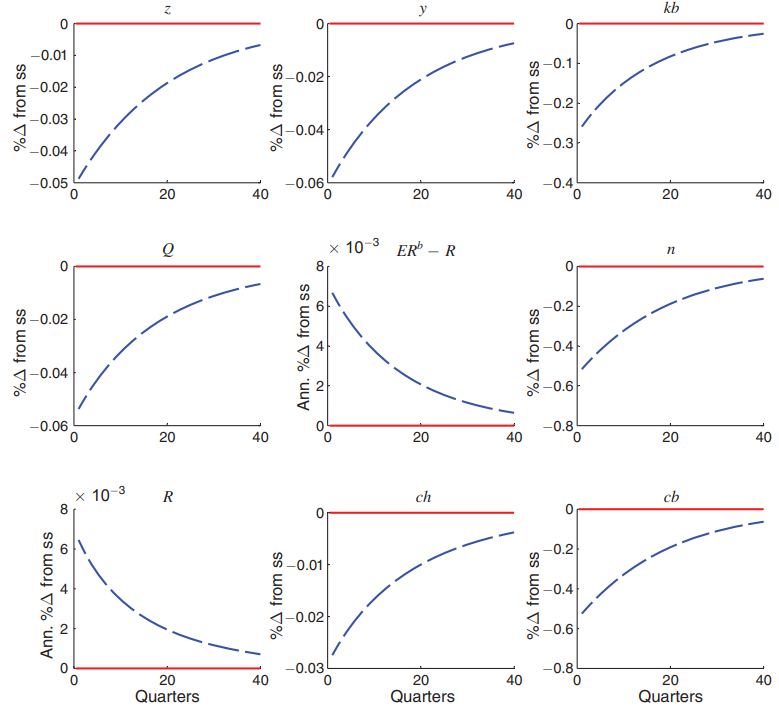
\includegraphics[height = 0.9\textheight]{fig/fig3.png}
        \caption{A Recession in the Baseline Model: No Bank Run Case}
    \end{figure}
\end{frame}

\begin{frame}
    \begin{figure}
        \centering
        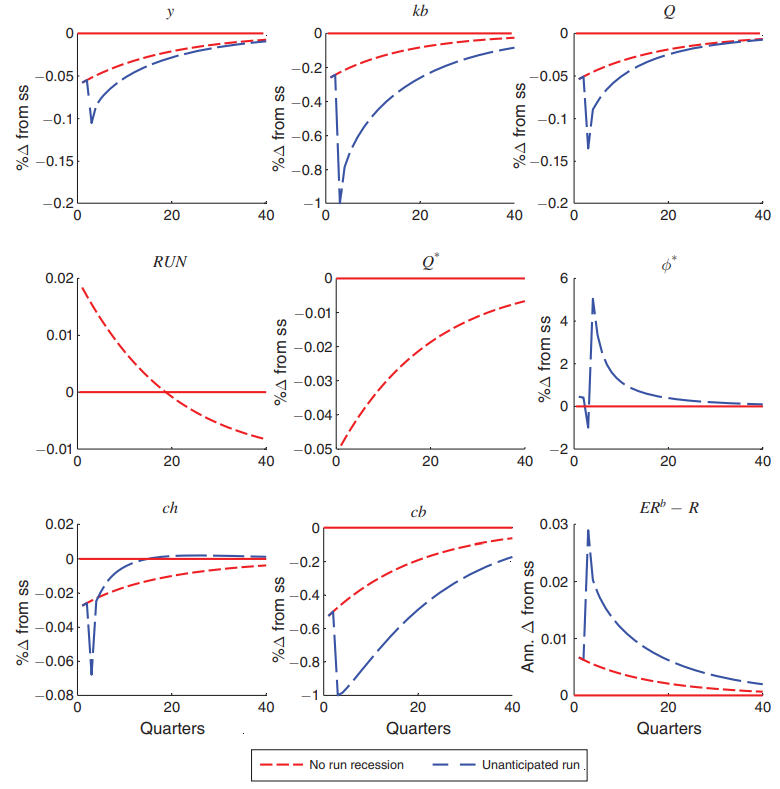
\includegraphics[height = 0.9\textheight]{fig/fig4.png}
        \caption{Ex Post Bank Run in the Baseline Model}
    \end{figure}
\end{frame}

\begin{frame}
    \begin{figure}
        \centering
        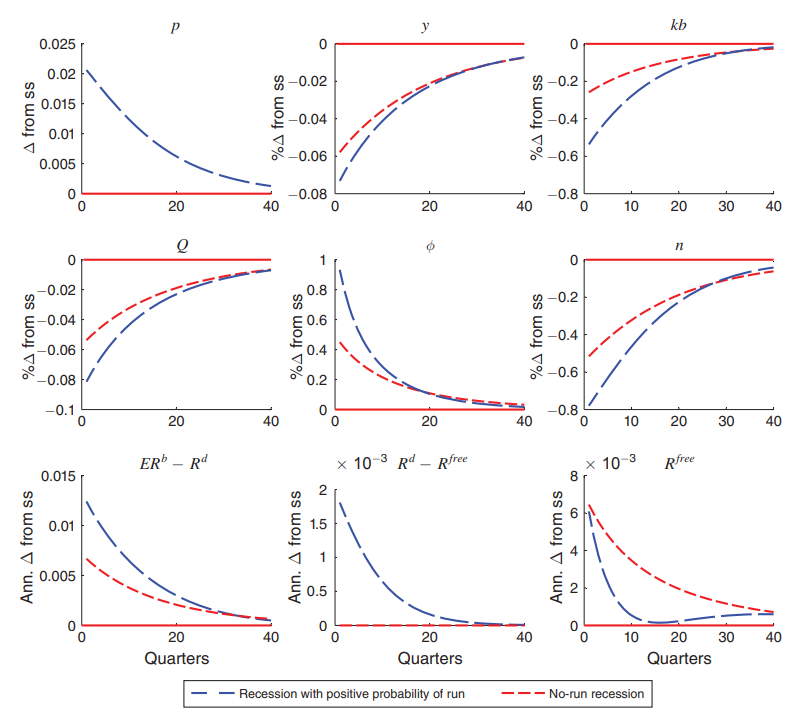
\includegraphics[height = 0.9\textheight]{fig/fig5.png}
        \caption{Recession with Positive Probability of a Run}
    \end{figure}
\end{frame}

\begin{frame}
    \begin{figure}
        \centering
        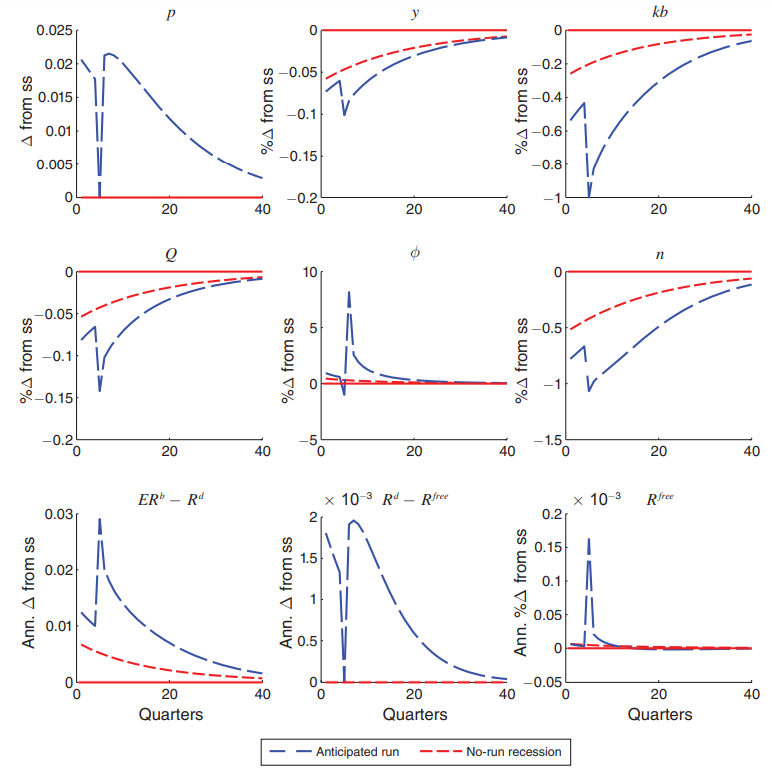
\includegraphics[height = 0.9\textheight]{fig/fig6.png}
        \caption{Recession with Positive Probability of a Run}
    \end{figure}
\end{frame}

\begin{frame}
    \begin{figure}
        \centering
        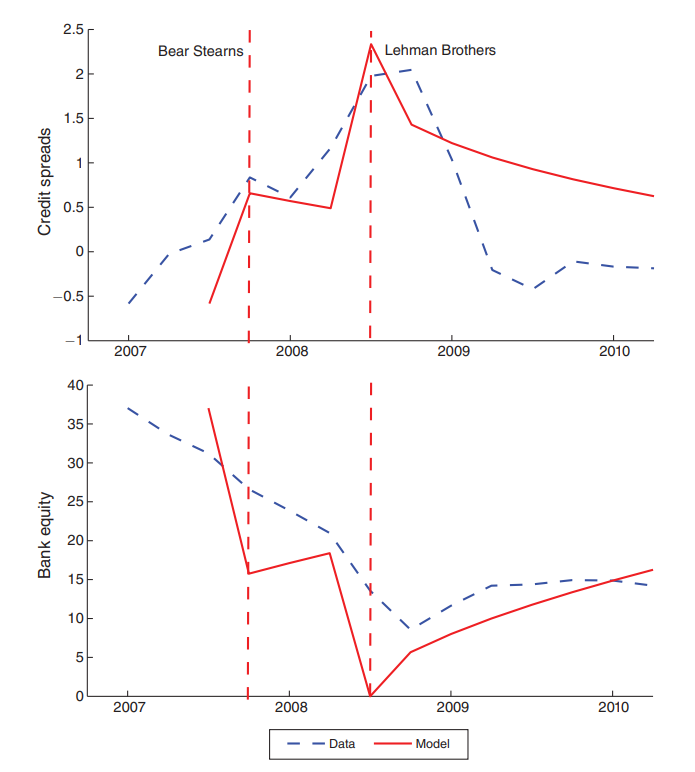
\includegraphics[height = 0.9\textheight]{fig/fig7.png}
        \caption{Recession with Positive Probability of a Run}
    \end{figure}
\end{frame}
\end{document}